\section{Optimising Abstract Graph Size}
\par \indent
As we have observed in lemmas \ref{aha-lemma:maxedgesincluster} and \ref{aha-lemma:maxtransitions} the initial abstraction algorithm attempts to represent every optimal path between clusters and inside clusters. 
However, while studying this problem we were unable to concot any scenarios where the number of edges is equal to the the theoretical worst-case suggesting that it is, infact, just an approximate upper-bound.  
A more exact characterisation is not easily derived due mostly to the combinatorial blow-up of possible terrain arrangements on even small maps with highly limited variable domains.
\par \indent 
A consequence of this observation is that in all experimental scenarios the same path was often returned for different pairs of $(c, s)$ parameters when using AA* to discover intra-edges. We highlight the problem in figure \ref{aha-fig:strongdominance}(a) and contrast it with our desired result in \ref{aha-fig:strongdominance}(b). $\lbrace E3, E5 \rbrace$ represent the same path between nodes $b$ and $c$ but are annotated with different clearance values. The same problem is evident for $\lbrace E4, E6 \rbrace$ which both cover nodes $a$ and $c$. In such cases we say that $E3$ and $E4$ are \emph{strongly dominant}, which we denote $E3 \prec E5$ and $E4 \prec E6$. We give the following definition to formalise this concept:

\begin{theorem}
\label{aha-definition:strongdominance}
Let $e_{a}, e_{b} \in E_{abs}$ be two edges that connect the same pair of abstract nodes. 
Assume both edges are traversable by a common capability with clearance such that $e_{a}(c), e_{b}(c) > 0$ where $c \in C \wedge c \neq \emptyset$. Then $e_{a} \prec e_{b}$ iff
$$ 1 \geq e_{a}(c) \geq e_{b}(c) \wedge weight(e_{a}) \leq weight(e_{b})$$
\end{theorem}

We term the resultant graph in which all strongly dominant edges have been removed a \emph{high-quality} abstraction.  
In figure \ref{aha-fig:abstractgraph}(c) we can see the complete graph for our running example; we were able to represent a 2-terrain map with 100 nodes and 350 edges using just 15 nodes and  37 edges. 

\begin{figure}[htbp]
        \caption{\emph{Strong edge dominance} }
        \begin{center}
                        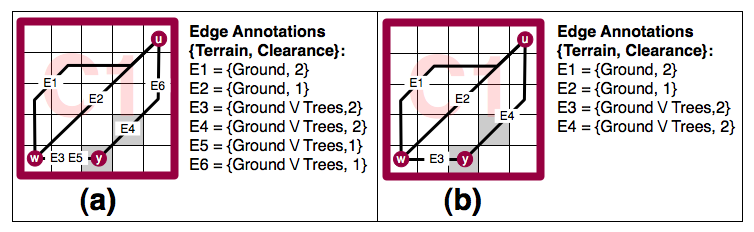
\includegraphics[scale=0.3]{diagrams/intraedges_initial.png}
        \end{center}
        \label{aha-fig:strongdominance}
\end{figure}

The abstract graph can be further reduced by noticing that some multi-terrain transitions between clusters can be removed without affecting the completeness of the representation. 
Figure \ref{aha-fig:abstractgraph}(a) and (b) highlight the problem and \ref{aha-fig:abstractgraph}(c) and (d) the desired outcome.
In this example we can see that although edges $E1$ and $E2$ have different clearance values any agent of size $s \in S : S = \lbrace 1, 2 \rbrace$ capable of traversing $E2$ can also traverse $E1$ without loss of generality. 
In such cases we say $E1$ is \emph{weakly dominant} and denote it as $E1 \sim E2$. 
We may further notice that $E3 \sim E4$, $E6 \sim E7$, $E10 \sim E8$ and $E10 \sim E9$ which suggests we can safely remove the dominated edges without losing any connectivity information from the graph. 
We formalise the concept using the following theorem:
\begin{theorem}
\label{aha-theorem:weakdominance}
Let $(n1_{a}, n2_{a}), (n1_{b}, n2_{b}) \in V_{abs}$ denote two pairs of abstract nodes in two adjacent clusters $\lbrace L_{1}, L_{2} \rbrace$ each covered covered by an inter edge $e_{a}, e_{b} \in E_{abs}$ with clearance values $e_{a}(c_{a}), e_{b}(c_{b})  : c_{a}, c_{b} \in C$.
 In this scenario, $e_{a} \sim e_{b}$ iff the following conditions are met:
\begin{enumerate}
\item{The capability dominance condition: $e_{a}(c_{b}) \geq e_{b}(c_{b})$}
\item{The circuit condition: $\exists intra_{1}, intra_{2} \in E_{abs} : (n1_{a}, n1_{b}) \in intra_{1} \wedge (n2_{a}, n2_{b}) \in intra_{2} \wedge intra_{1}(c_{b}) \geq e_{b}(c_{b}) \wedge intra_{2}(c_{b}) \geq e_{b}(c_{b})$.}
\end{enumerate}
Then, any location which an agent can reached by traversing $e_{b}$ can also be reached by $e_{a}$.
\end{theorem}

\begin{proof}
If a circuit exists between the endpoints $\lbrace n1_{a}, n2_{a}, n1_{b}, n2_{b} \rbrace$ which contains only edges with clearances at least as large as $e_{b}(c_{b})$ for the capability $c_{b}$ then any nodes which are reachable from $n1_{b}$ or $n2_{b}$ are also reachable from $n1_{a}$ or $n2_{a}$.
From this it follows that any destination an agent can reach via $e_{b}$ can also be reached via $e_{a}$ 
\end{proof}
The number of edges which are weakly dominated can be maximised by leveraging the fact that there are only a limited number of sizes agents may take. We can thus apply the following truncation condition to the abstract graph before we apply weak dominance:
\begin{equation}
e(c) > max(s) \Rightarrow e(c) = max(s) : s \in S, \forall e \in E_{abs}
\end{equation}
\par \indent
A direct consequence of theorem \ref{aha-theorem:weakdominance} is that in addition to removing weakly dominated inter-edges, we can also remove their endpoints and any intra edges dependent on those nodes; by the circuit condition, these are also dominated. 
This corrolary only applies if the endpoints are not required by another (non-dominated) inter-edge representing a different cluster transition. 
\par \indent
We refer to the initial abstraction that has had both strong and weakly dominated edges removed a \emph{low quality abstraction}.
In \ref{aha-fig:abstractgraph}(c) we reduce the high quality abstraction from \ref{aha-fig:abstractgraph}(a) to 10 nodes and 13 edges.
\begin{figure}[htbp]
        \caption{\emph{High and low quality abstraction results} }
        \begin{center}
                        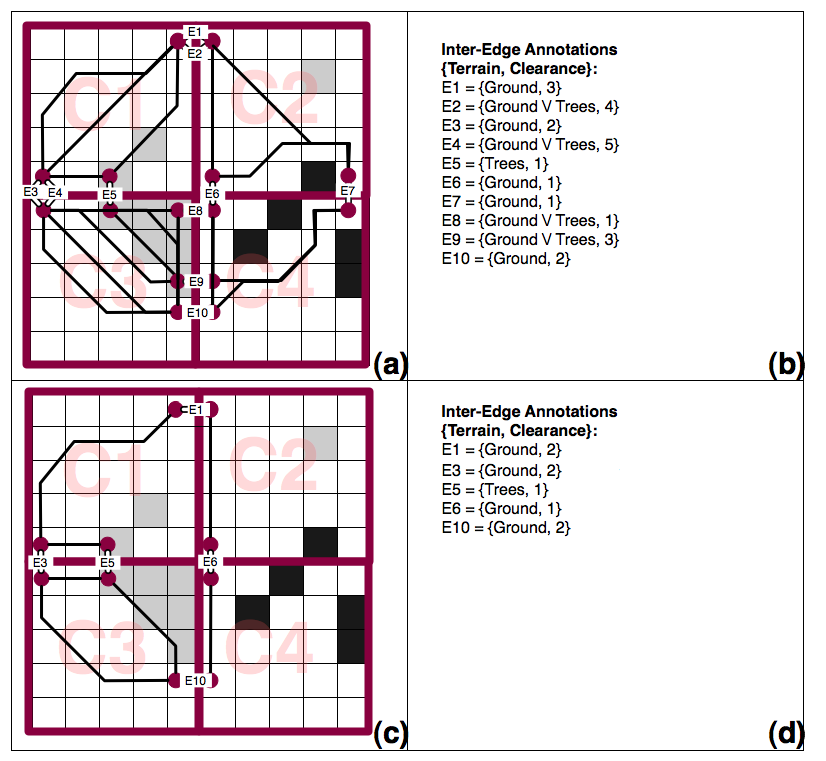
\includegraphics[scale=0.25]{diagrams/abstraction_result.png}
        \end{center}
        \label{aha-fig:abstractgraph}
\end{figure}
\par \indent
A reasonable analogy to highlight the intuition behind theorem \ref{aha-theorem:weakdominance} is to compare the way off-road vehicles opportunistically use roads where possible even if an off-road route (or trail) might exist which has a smaller distance cost. Roads are smoother to drive on and have other benefits such less wear and tear, and better fuel consumption. Opting for a lower-quality abstraction in this way does have an effect on the quality of the computed solutions, but as we will show, the differences are reasonably small and the solutions still near-optimal. The best choice depends on the requirements of the specific application to which the algorithm is applied; it is a classic tradeoff between performance vs space.
\par \indent
Regardless of the choice however, both types of dominance retain representational completeness and guarantee solutions for all valid problems.


